
%%%%%%%% Prelude Start %%%%%%%
 
% \IEEEPARstart{T}{o} establish a ubiquitous Internet of Things (IoT), tens of billions of devices are to be installed, and possibly at hard-to-reach locations~\cite{6064380, 7347318, 7954016, 7488250}. 
% Using non-rechargeable batteries constrains the lifespan of these devices and brings impractical battery replacement work. 
% Enabling IoT devices to harvest ambient energy becomes a solution to circumvent the limited battery lifespan. 

% --- paper ---
% Internet of Things (IoT) devices are becoming ubiquitous, with forecasts of hundreds of billions being installed in the near future~\cite{sparks2017trillion}.
% ~\cite{7954016, sundmaeker2010vision, dave2011next} % old citations for predictions 
% ~\cite{6064380, 7347318, 7954016, 7488250}. 
% They are conventionally battery-powered, thus have constrained lifespans, necessitating inconvenient periodic battery replacement.
% Energy-harvesting is a potential solution. Environmentally harvested power is, however, intrinsically variable and intermittent~\cite{4494336}. Traditionally, large energy storage devices such as rechargeable batteries or supercapacitors are used to smooth out supply variability~\cite{Kansal:2007:PME:1274858.1274870}. Unfortunately, these increase cost and device dimensions~\cite{4494753}, raise pollution concerns~\cite{LIU2014210}, and still limit lifespans~\cite{AKHTAR2015769}. 
% --- paper ---

% yet using an energy-harvesting supply without energy buffering hinders execution by frequent power interruptions. 
% Buchli:2014:DPM:2668332.2668333, Wagemann:2017:OER:3136518.3078631,
% ~\cite{5522465, Kansal:2007:PME:1274858.1274870, Jiang:2005:PEP:1147685.1147765, Simjee:2006:ELS:1165573.1165619}

%%%%%%%%%%%%%%%%%%%%%%
% Recent research has developed \textit{intermittent computing} for energy harvesting devices to maintain execution despite frequent power interruptions by saving and restoring system volatile computing state through non-volatile memory (NVM)~\cite{Ransford:2011:MSS:1950365.1950386, 10.1145/2700249, 6960060, Lucia:2015:SSP:2737924.2737978, 6341281}. 
% % In particular, if the supply voltage is charged above a restore threshold, such systems wake up and execute. 
% During active periods, the systems save volatile state (e.g. CPU registers, RAM data) into NVM either at pre-installed points (\textit{static}) or when the supply is about to fail (\textit{reactive}). If the supply voltage drops below the minimum operating threshold, the systems lose all volatile state and shut down, with data in NVM preserved. After the supply voltage recovers to a restore threshold, the systems restore the saved state from NVM and continue execution from the last saved point. Thereby, despite frequent supply interruptions, forward execution is preserved without large energy storage. 
%%%%%%%%%%%%%%%%%%%%%%

% To remove large energy storage while maintain execution despite frequent power interruptions, recent research has developed \textit{intermittent computing} (also known as \textit{intermittent computing}), which saves and restores system volatile computing state (e.g. CPU register data, RAM data) through nonvolatile memory (NVM)~\cite{Ransford:2011:MSS:1950365.1950386, 10.1145/2700249, 6960060, Lucia:2015:SSP:2737924.2737978, 6341281, 199319}. During active periods, the system volatile state is saved into NVM either at pre-installed points (\textit{static}) or just before the power supply fails (\textit{reactive})~\cite{sliper2019efficient}. The volatile state is lost when the supply voltage drops below the minimum operating threshold, while the saved state in NVM is retained. The saved state is restored from NVM when the supply voltage recovers to a restore threshold, and then the execution continues from the last saved point. Therefore, forward execution is preserved without large energy storage despite frequent supply interruptions. In intermittent computing, forward progress denotes the effective program progress, as opposed to re-executed progress, lost progress, and the progress of state-saving and -restoring operations~\cite{7478428, 7056060}. The amount of forward progress directly determines application performance (e.g. program iteration rate or task completion time). 
%%%%%%%%%%%%%%%%%%%%%%%

% --- paper ---
% Recently, \textit{intermittent computing systems} (IPSs) have been proposed as an alternative~\cite{doi:10.1098/rsta.2019.0158}. Instead of using large energy storage devices to sustain execution, they tolerate power interruptions by saving the state of the system into non-volatile memory (NVM) so that computation can continue when power is restored. They may save this state (e.g. CPU registers and RAM contents) either \textit{statically} at pre-defined points, or \textit{reactively} by detecting when the supply is about to fail~\cite{doi:10.1098/rsta.2019.0158}.
% --- paper ---
% ~\cite{Ransford:2011:MSS:1950365.1950386, 10.1145/2700249, 6960060, Lucia:2015:SSP:2737924.2737978, 6341281, 199319}

%%%%%%%% Prelude End %%%%%%%




%%%%%%%% IPS Review Start %%%%%%%

% --- paper ---
% Static IPS approaches save state at points determined at design or compile time, either by inserting checkpoints~\cite{Ransford:2011:MSS:1950365.1950386, 7944791} or decomposing a program into atomic tasks\footnote{Atomic operations in IPSs denote operations that should be completed in one continuous period. 
% If an atomic operation is interrupted by a power failure, it should be re-executed rather than resumed. Examples of atomic operations include saving and restoring volatile state, transmitting and receiving packets, and sampling sequences of data from sensors.}~\cite{10.1145/3360285, Maeng:2017:AIE:3152284.3133920}. 
% After a power interruption, progress rolls back and resumes from the last saved checkpoint or task boundary. This can introduce issues such as violation of data memory consistency, along with wasting energy on lost and re-executed progress.

% Conversely, reactive IPS approaches monitor the supply voltage and only save state when it falls below a threshold~\cite{balsamo2016hibernus++, 7849206, 7807254}, which is set high enough to reliably save state even with a total and immediate drop-off in harvested energy. 
% They then enter a low-power mode, in many cases preserving their volatile memory and avoiding re-execution. These typically make more forward progress than static approaches, e.g. a 2.5$\times$ mean computational speedup~\cite{Maeng:2019:SPI:3314221.3314613}. 
% --- paper ---


% Advantages include minimising hardware dependency, and ensuring operation atomicity.However, progress rollback and re-execution
% Static approaches save volatile state into NVM at points determined at design time or compile time, either by inserting checkpoints~\cite{Ransford:2011:MSS:1950365.1950386, 7944791, 222579} or decomposing a program into atomic tasks~\cite{10.1145/3022671.2983995, Maeng:2017:AIE:3152284.3133920}. After power interruptions, the progress rolls back and resumes from the last saved checkpoint or task boundary. Advantages of static approaches include minimizing hardware dependency and ensuring operation atomicity. However, the progress rollback and re-execution introduce violation of data memory consistency, and waste energy on lost and re-executed progress. 
% % Also, if the consumption between two successive checkpoints or task boundaries exceeds the amount that the energy storage can guarantee, the progress may never proceed due to insufficient power input. 



% and memory inconsistency
% In contrast to static approaches, reactive approaches only save volatile state in NVM when supply is about to fail by monitoring supply voltage~\cite{10.1145/2700249, 6960060}. Specifically, a reactive IPS saves volatile state and enters a low-power mode (execution halted) if the supply voltage falls below a save threshold. This save threshold is set high enough to successfully save volatile state before power fails. 
% By entering the low-power mode, reactive approaches avoid re-execution and memory inconsistency, and hence typically make more forward progress than static approaches, e.g. a 2.5$\times$ mean computational speedup presented in~\cite{Maeng:2019:SPI:3314221.3314613}. 
% % In a comparison between static~\cite{Maeng:2017:AIE:3152284.3133920} and reactive~\cite{10.1145/2700249} approaches, the reactive approach demonstrates a 2.5$\times$ mean speedup on computational workloads~\cite{Maeng:2019:SPI:3314221.3314613}. Therefore, we focus on reactive IPSs for modelling and validation in this paper. 


%system computing state, e.g. CPU registers and RAM contents, into nonvolatile memory (NVM). either at pre-installed points (\textit{static methods}) or when the supply is about to fail (\textit{reactive methods})~\cite{sliper2019efficient, doi:10.1098/rsta.2019.0158}. 
% The volatile state is lost when the supply voltage drops below the minimum operating threshold, while the saved state in NVM is retained. The saved state is restored from NVM when the supply voltage recovers to a restore threshold, and then the execution continues from the last saved point. 
% Therefore, forward execution is preserved. 

%%%%%%%% IPS Review End %%%%%%%






%%%%%%%%%%%%%%%%%%%%%%%
% turn into the main topic now: modelling progress, improvement by sizing energy storage 
%%%%%%%%%%%%%%%%%%%%%%%

% Modelling and estimating forward progress of an energy-harvesting intermittent computing (EHIC) device is crucial to evaluation of whether the device can achieve expected performance with variable energy source conditions after deployment, while requires considerations on energy source variability and understanding of intermittent computing systems. 
% However, traditional computer models are not able to achieve this due to lack of considerations on energy source variability and understanding of intermittent computing systems. 

% What we did? What we did differently from them?
% We provide a modelling approach to estimate forward progress of an IPS in real-world deployment, considering energy source conditions as well as the forward progressing behaviours intermittent computing. This model can be used to explore the effect of energy harvester and energy storage sizing on forward progress. Further, we provide an approach for sizing energy storage in intermittent systems. 

With the goal of minimising device dimensions and interruption periods, most IPS approaches adopt only a minimum amount of energy storage~\cite{balsamo2016hibernus++, 10.1145/2700249, 10.1145/2809695.2809707, 10.1145/3281300, 222579, 7403941, 10.1145/3281300}, e.g. a decoupling capacitor. 
This is typically just sufficient for the most energy-expensive atomic operation. 
However, our assertion is that this can be \textit{inherently inefficient in terms of time and energy}. 
We show that a system with minimum energy storage frequently goes through a cycle of: wake up, restore state, execute program, save state, and halt.
We propose that provisioning \textit{slightly more} energy storage can prolong the operating cycles, reduce the frequency of interruptions, and hence improve forward progress. 
We show with modelled and experimental results that (\fref{fig:imprvalid1}) using efficiently-sized energy storage capacitance (\SI{43}{\micro\farad}) achieves up to a 55\% improvement in forward progress compared against using the theoretical minimum amount of capacitance (\SI{6.2}{\micro\farad}). 
This improvement is more significant with a weaker supply. 

\begin{figure}
    \centering
    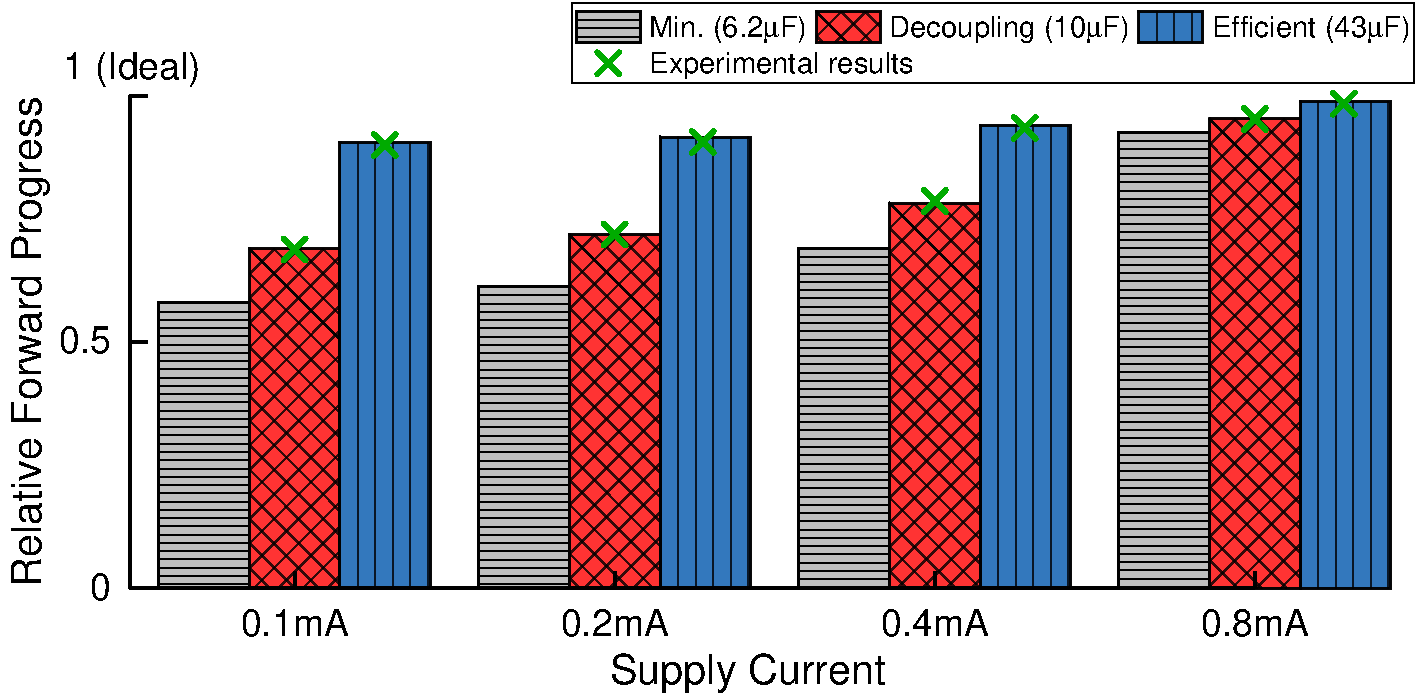
\includegraphics[width=0.8\columnwidth]{ch3_sizingeffect/figures/ImprValidColorFig1}
    \caption{The relationship between energy storage capacitance and IPS forward progress, for various supply currents. }
    \label{fig:imprvalid1}
\end{figure}

% However, larger energy storage also increases leakage current, occupies greater volume, and requires longer interruption periods. 
% We further propose an approach for identifying the proper energy storage size for deploying energy-harvesting intermittent computing (EHIC) devices, which improves forward progress while balances dimensions and interruption periods. We integrate the reactive intermittent computing model into a photovoltaic-based (PV-based) EHIC device framework. We demonstrate the sizing approach with the framework given various real-world indoor and outdoor light source datasets. 

However, the relationship between IPS energy storage capacitance and forward progress has not previously been defined.
Due to the computational speedup of reactive IPSs over proactive IPSs as discussed in \sref{Chapter:Review}, we focus on reactive IPSs in this chapter. 
We develop an experimentally-validated model of reactive IPSs to estimate forward progress. 
Taking advantage of the theoretical model, we explore the effect of energy storage capacitance on forward progress with respect to supply current and volatile state size. 
The main contributions in this chapter can be summarised as:
\begin{itemize}
    \item A reactive IPS model which accurately estimates forward progress; experimental validation shows a 0.5\% mean error. 
	\item An exploration based on the model, where we analyse the energy storage sizing effect on forward progress with respect to supply current and volatile state size, showing up to 65\% forward progress improvement.
    % while reduces capacitor volume by \SI{71.7}{\percent} and interruption periods by \SI{83.8}{\percent} as simulated with real energy availability data (Section~\ref{section:demo}). 
    % that trades off forward progress, capacitor volume, and interruption periods in IPSs . 
    % compared to solely maximising forward progress in simulations.%\footnote{). 
%    \color{black}
    % \item A demonstration of the sizing approach with the theoretical model integrated into a photovoltaic-based (PV-based) IPS model under various real-world light source datasets, where the suggested capacitance achieves \SI{98.3}{\percent} of the maximum forward progress while saves \SI{71.7}{\percent} capacitor volume and \SI{83.8}{\percent} interruption periods (Section~\ref{section:demo}). 
    % results show that sizing energy storage can improve annual mean forward progress by \SIrange{7.8}{43.3}{\percent}.

    % \item Experimental validation of the theoretical model, which shows high accuracy with \SI{0.5}{\percent} mean absolute percentage error, and a \SI{43}{\micro\farad} capacitor suggested by the sizing approach improves forward progress by up to \SI{55.2}{\percent} and \SI{30.4}{\percent} compared to a theoretical minimum \SI{6.2}{\micro\farad} one and an on-board \SI{10}{\micro\farad} one across various levels of supply current. 

    % \item where we found that a properly sized capacitor results in up to 30.4\% more forward progress in experiment compared to an on-board one, and improves mean forward progress by up to 35.0\% over one-year indoor and outdoor light energy harvesting simulation compared to a minimum one. 
    
    % \item experiments: which was experimentally validated with accuracy of 0.5\% mean absolute percentage error across various current input. 

    % \item We validate our formulation and model via experiments based on a TI MSP430FR6989 microcontroller, where the results show that 
\end{itemize}
%\color{blue}
% While most IPSs are designed with a minimal amount of energy storage, 
The associated simulation tool, coded in C, is available open-source~\footnote{\url{https://git.soton.ac.uk/energy-driven/energy-storage-sizing}}. %} with real energy availability data (Section~\ref{section:demo}

As discussed in \cref{Chapter:Introduction}, \textit{forward progress} denotes the effective application progress, excluding re-executed progress, lost progress, and state-saving and -restoring operations~\cite{7478428}. 
The amount of forward progress directly determines application performance, e.g. program iteration rate or task completion time. 
In this chapter, to allow fair comparison, we define normalised forward progress as \textit{the ratio of the effective execution time to the total elapsed time}, without being restricted to a specific workload. 

% (Section~\ref{section:exploration})
The rest of this chapter is organised as follows. 
The reactive IPS model is proposed in \sref{sec:c3_model}.
The exploration on the energy storage sizing effect is presented in \sref{section:exploration}.
\sref{sec:c3_experiment} validates the proposed model and the energy storage sizing effect. 
Finally, \sref{sec:c3_summary} summarises this chapter. 


% Design considerations: forward progress, energy storage, energy harvester
% Design specifications in intermittent computing devices typically focus on three things according to applications: forward progress, interruption periods, and device dimensions. 
% interruption periods denotes the time required to wake up the device when there is power available. In some event-driven applications, interruption periods should be reduced to ensure timely event handling. Device dimensions are restricted in some size-constrained applications, for example, wearable devices or in-body sensing. Sizing energy harvester and energy storage impacts these design specifications. 

% Besides energy storage, the size of energy harvester dominates the harvested power scale. Oversized energy harvester unnecessarily increases device costs, providing excess energy beyond the necessary amount to satisfy forward progress requirement. However, there is not a method for designers to seek a cost-efficient energy harvester size to meet their design specifications in real-world deployment. 

% A general problem statement. A general summary of this work. 
% In the deployment of intermittent computing devices, it is a challenge for designers to determine the sizes of energy harvester and energy storage to both satisfy application specifications and achieve cost-efficiency. 
% perhaps explain this cost-efficiency somewhere before this place, say that using minimum storage require perhaps a large energy harvester to achieve the performance spec, but increasing storage reduce that cost without dimensional penalty. 
% In this paper, we propose a modelling approach to explore the design space in sizing energy harvester and energy storage in the deployment of intermittent computing devices. 
